\subsection{ESP32 e MicroPython}
ESP32 è una famiglia di microcontrollori prodotta da espressif, con l'enorme
vantaggio di avere a bordo un modulo per la connettività Wi-Fi e Bluetooth, che
la rende ottima per lo sviluppo di sistemi IoT.

Ne esitono diversi modelli con specifiche tecniche leggermente differenti e sono
inoltre disponibili svariate schede che mirano a renderne l'utilizzo,
soprattutto in fase di progettazione, il più semplice possibile, integrando
sistemi di alimentazione e programmazione tramite USB e rendendola compatibile
con la tecnologia THT.


\begin{figure}[H]%
    \centering
    \begin{subfigure}{0.49\textwidth}
        \centering
        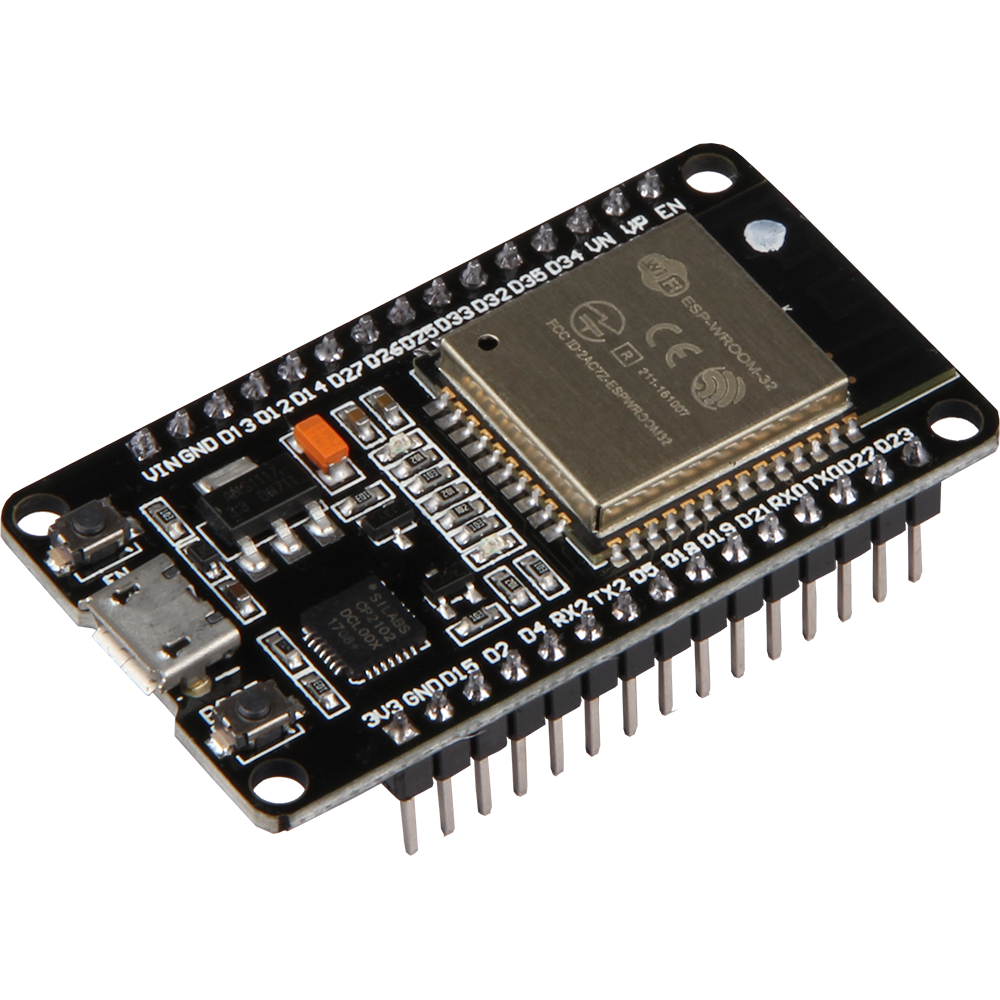
\includegraphics[scale=0.4]{introduzione/esp32.png}%
        \caption{Scheda basata su ESP32}
    \end{subfigure}
    \begin{subfigure}{0.49\textwidth}
        \centering
        \caption{Caratteristiche tecniche di base}
        \begin{tabular}{|c|c|}
            \hline
            Internal clock frequency & 40MHz        \\
            \hline
            Ram                      & 520Kb        \\
            \hline
            Rom                      & 480Kb        \\
            \hline
            SPI Flash memory         & 4/8/16 Mb    \\
            \hline
            Supply voltage           & 3.0 to 3.6 V \\
            \hline
        \end{tabular}
    \end{subfigure}
    \caption{Esempio di ESP32}
\end{figure}

L'hardware più moderno e prestante rispetto ad altri microcontrollori rendono
ESP32 un'ottima scelta per quanto riguarda l'utilizzo di MicroPython, un
firmware particolare che una volta caricato sulla scheda ne permette la
programmazione tramite un linguaggio interpretato quasi totalmente compatibile
con l'implementazione x86 di Python.